\chapter{Experiments \& Results}

The current raptor code in Dash is only developed for replacing \texttt{getdata} requests.
We have compared 2 metrics in order to compare the techniques. The results shown
below can efficiently be applied to compact blocks, XThin and Graphene blocks in
cases where the block transactions are sent.

\section{Evaluation Criteria}

\begin{enumerate}
    \item The orphan rate. The orphan rate tells us how many blocks weren’t
    added to the block and how much profitable it will be for a miner to use
    this technique.
    \item The block propagation times for median block propagation on
    of the nodes.  
        The block sizes we have used are from 100MB to 1GB.
    \item Orphan rates for different symbol sizes help us understand what symbol
        size to use.

\end{enumerate}

Below is a detail of all the experiments that were run in order to test the
hypothesis and understand the implications of introducing Fountain Codes into
the current state of blockchains.

\section{Dash Core Client}
\subsection{Testing Environment}
\begin{enumerate}
    \item DashCore version 12.3 is used for development.
    \item libRaptorQ \citep{libraptor} 0.1.X branch, 697b318036a1ea4751e69cde7989ff3b3bd7c655
    commit is used. The code needs to be changed in order to directly include
    the header files. 
    \item 3 local nodes in regression test mode were spawned for each
    experiment.
    \item Each node creates its own blockchain in the assigned directory.
\end{enumerate}

The tests done on the actual dash core client were used to find out how many
repair symbols were used in order to complete the data.

\subsection{Observations}
\begin{enumerate}
    \item It was observed, that for a block on regression
        test mode, the aggregated size of \texttt{k} encoded symbols had the same size as that of a block mined.
    \item In the setup of 3 nodes and 4 nodes, we sent 1/3 and 1/4 encoded
        symbols from each node to the receiving node and we were able to
        recreate the block.
    \item For small block sizes, we used 4 byte and 16 byte symbols. But for
        larger blocks, symbols can be as long as we want, with the constraint
        that symbol size is divisible by encoded array sent. If this is not the
        case, the decode fails. Therefore, symbol size and encoded vector size
        is negotiated in the \texttt{getraptor} request.
\end{enumerate}

\section{Dash Simulator}

\subsection{Testing Environment}

\begin{enumerate}
    \item The simulator is run with 24 nodes, with 8 mining pools. 8 full nodes 
        and 8 masternodes. 24 nodes here represent the whole network because:
        \begin{enumerate}
            \item For this protocol to work, memory pool synchronization is not required.
            \item Both traditional and the fountain protocol are compared on a 24 node network in order to have a fair comparison. 
            \item Traditional propagation is used, because the messages - \texttt{blocktxn}, \texttt{xblocktx} and \texttt{grblocktx} in compact, XThin and graphene respectively are similar to full blocks except they are smaller in size (Since only missing transactions are propagated}.
        \end{enumerate}
    \item The masternodes although in the real network have higher bandwidth, in 
        this experiment we have kept it the same as full nodes. The reason for this 
        is to extrapolate these results to other public cryptocurrencies.
    \item The average bandwidth taken for each node is taken from \citep{bandwidth},
        where the paper talks about the latency and the bandwidth distribution for 
        each continent.
    \item The simulations for run for 100 blocks each.
    \item Different symbol sizes have been used to understand the dependency of symbol sizes on orphan rate.
        \texttt{k} varies between 10 and 10000 i.e the number of symbols required to reconstruct the block. Orphan rates are calculated for each of these \texttt{k} to understand the ideal size for raptor code symbol size.
    \item Each node only forwards 50\% symbols, except the miners, who stream the
        all the symbols. In case if only one node is streaming the block, the data is re-requested and the rest 50\% are streamed.
    \item The average bandwidth distributions are taken from \citep{bandwidth} which for these simulations ranged below 50 MB per second.
\end{enumerate}

\begin{figure}
    \captionsetup{justification=centering}
    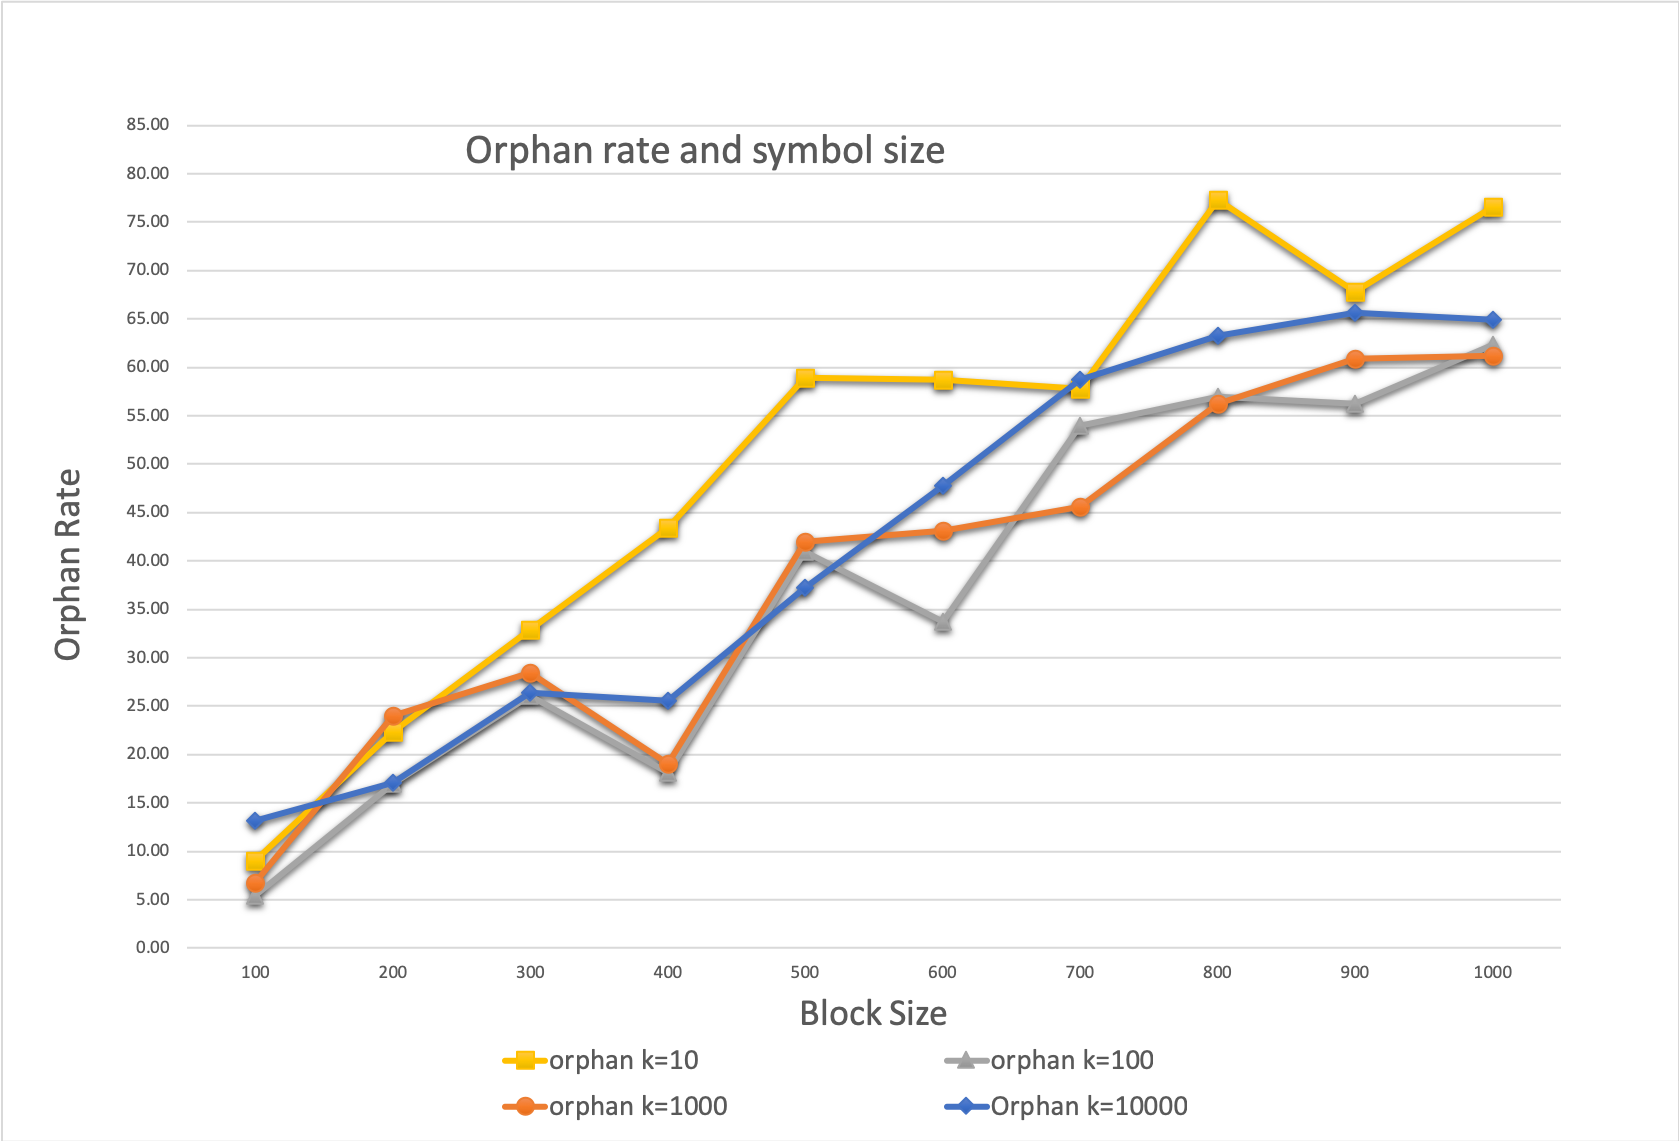
\includegraphics[width=1\columnwidth, height=.6\columnwidth]{files/symbolSize.png}
     \centering
     \caption{Orphan rate with respect to symbol Sizes }
     \label{image: symbol}
\end{figure}

\subsubsection{Choosing the symbol size}
In order to aggregate the symbols from the peer nodes, we need to understand what ratio of the block size should the symbol size be in order for the propagation to be optimal for the bandwidth of the nodes that we have tested.

The following are the observations based on \ref{image: symbol}. In the graph, \texttt{k} refers to the number of symbols required to reconstruct the block. All symbols are equal in size. 

\begin{enumerate}
    \item For $k = 10$, we see that for 100MB blocks although the orphan rate starts with a low value of 9\%, it increases fast as the block size increases. This is because the symbols sizes become larger than the upload bandwidth for the node and therefore take time to propagate. 

    \item For $k=100$ and $k=1000$ , the orphan rate increases at almost the same rate. It can be noticed that although the symbol sizes differ by a magnitude of 10, for block sizes between 100MB and 1000MB, symbols will vary between 1MB and 10MB, which are still not utilizing the complete bandwidth of the node and hence take lesser time to propagate and therefore less orphanage.

    \item For $k=10000$ in smaller block sizes, between 100MB and 400MB, the performance is optimal, although when the block sizes grow, it is seen that the orphan rate is similar to that of $k=100$ and $k=1000$, which is still significantly less than the original block propagation.

\end{enumerate}

\subsection{Results}

\subsubsection{Orphan Rates}

\begin{figure}
    \captionsetup{justification=centering}
    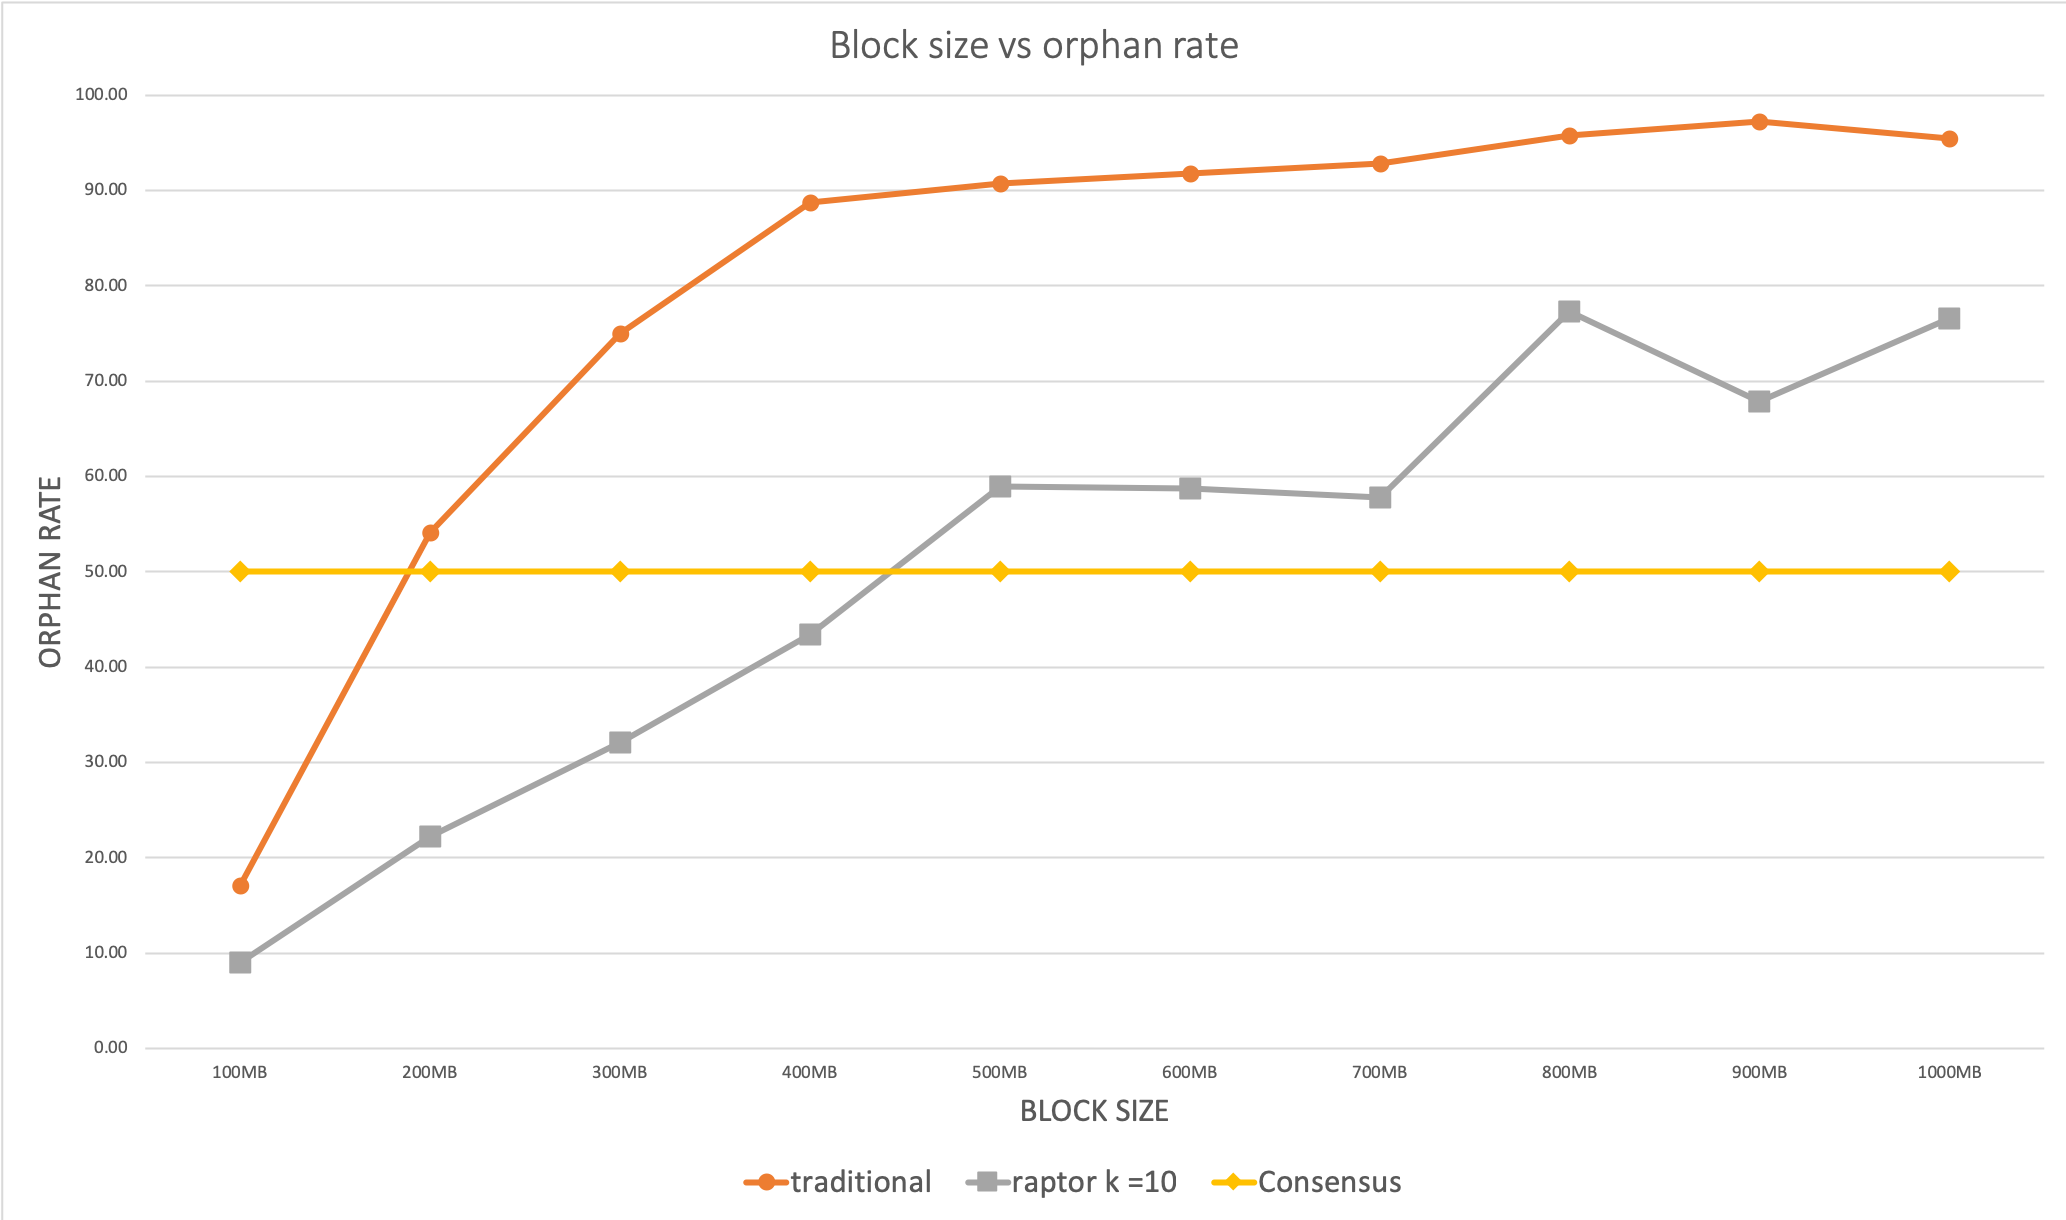
\includegraphics[width=1\columnwidth, height=.7\columnwidth]{files/orphan_10.png}
     \centering
     \caption{Block Size vs Orphan Rate k=10}
     \label{image: orphan_10}
\end{figure}

\begin{figure}
    \captionsetup{justification=centering}
    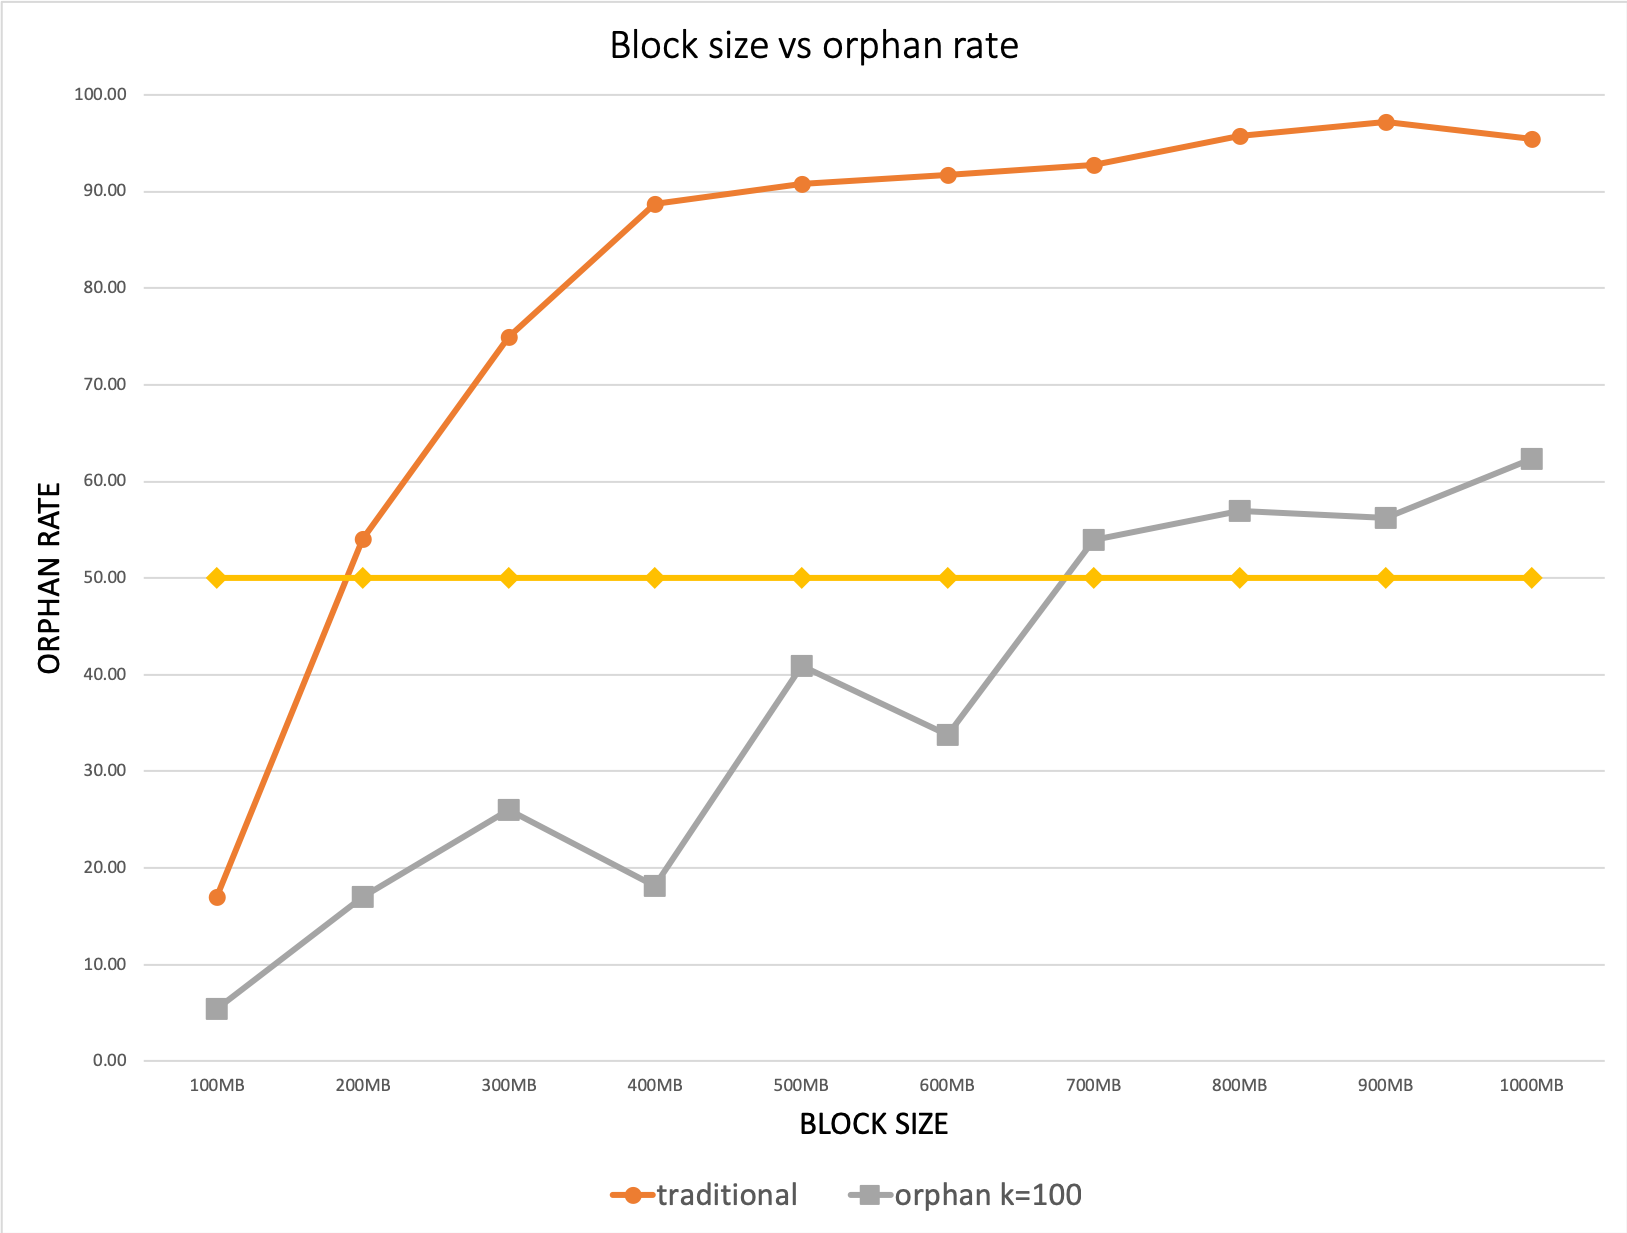
\includegraphics[width=1\columnwidth, height=.7\columnwidth]{files/orphan_100.png}
     \centering
     \caption{Block Size vs Orphan Rate k=100}
     \label{image: orphan_100}
\end{figure}

\begin{figure}
    \captionsetup{justification=centering}
    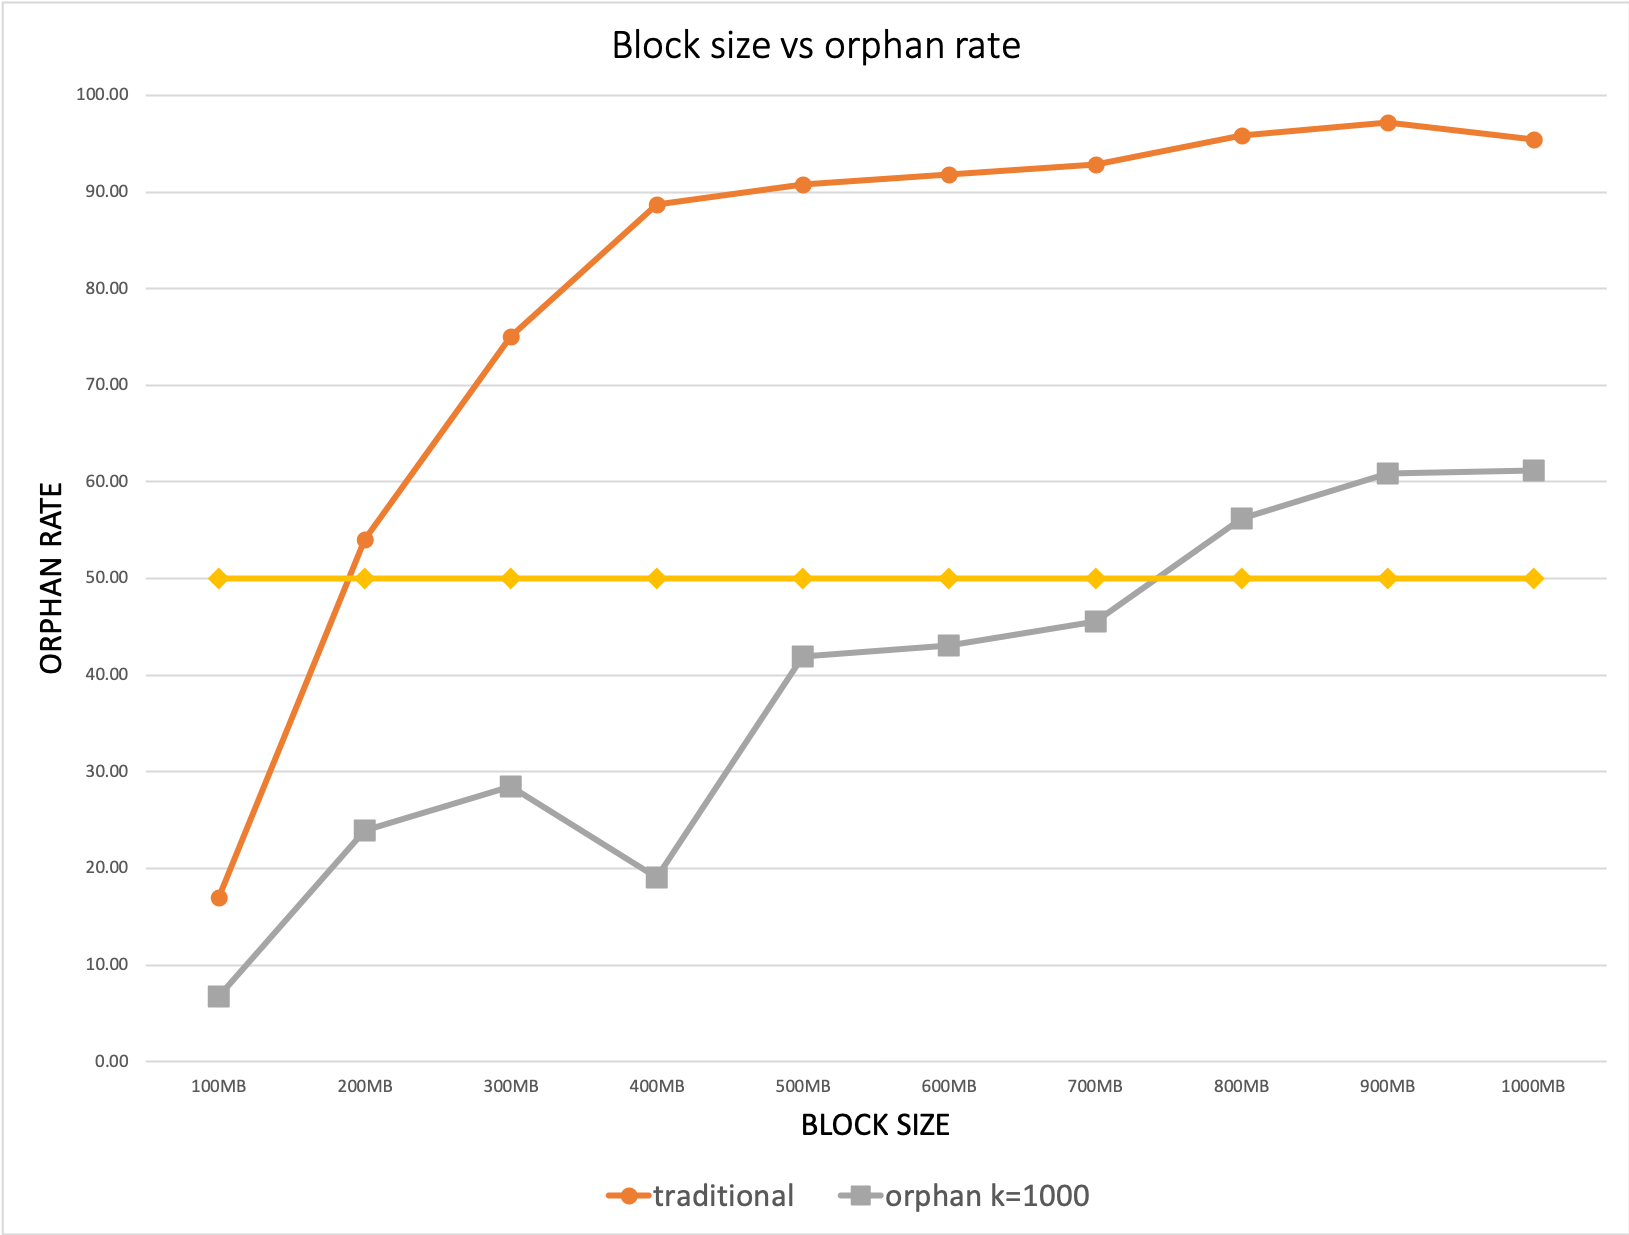
\includegraphics[width=1\columnwidth, height=.7\columnwidth]{files/orphan_1000.png}
     \centering
     \caption{Block Size vs Orphan Rate k=1000}
     \label{image: orphan_1000}
\end{figure}

\begin{figure}
    \captionsetup{justification=centering}
    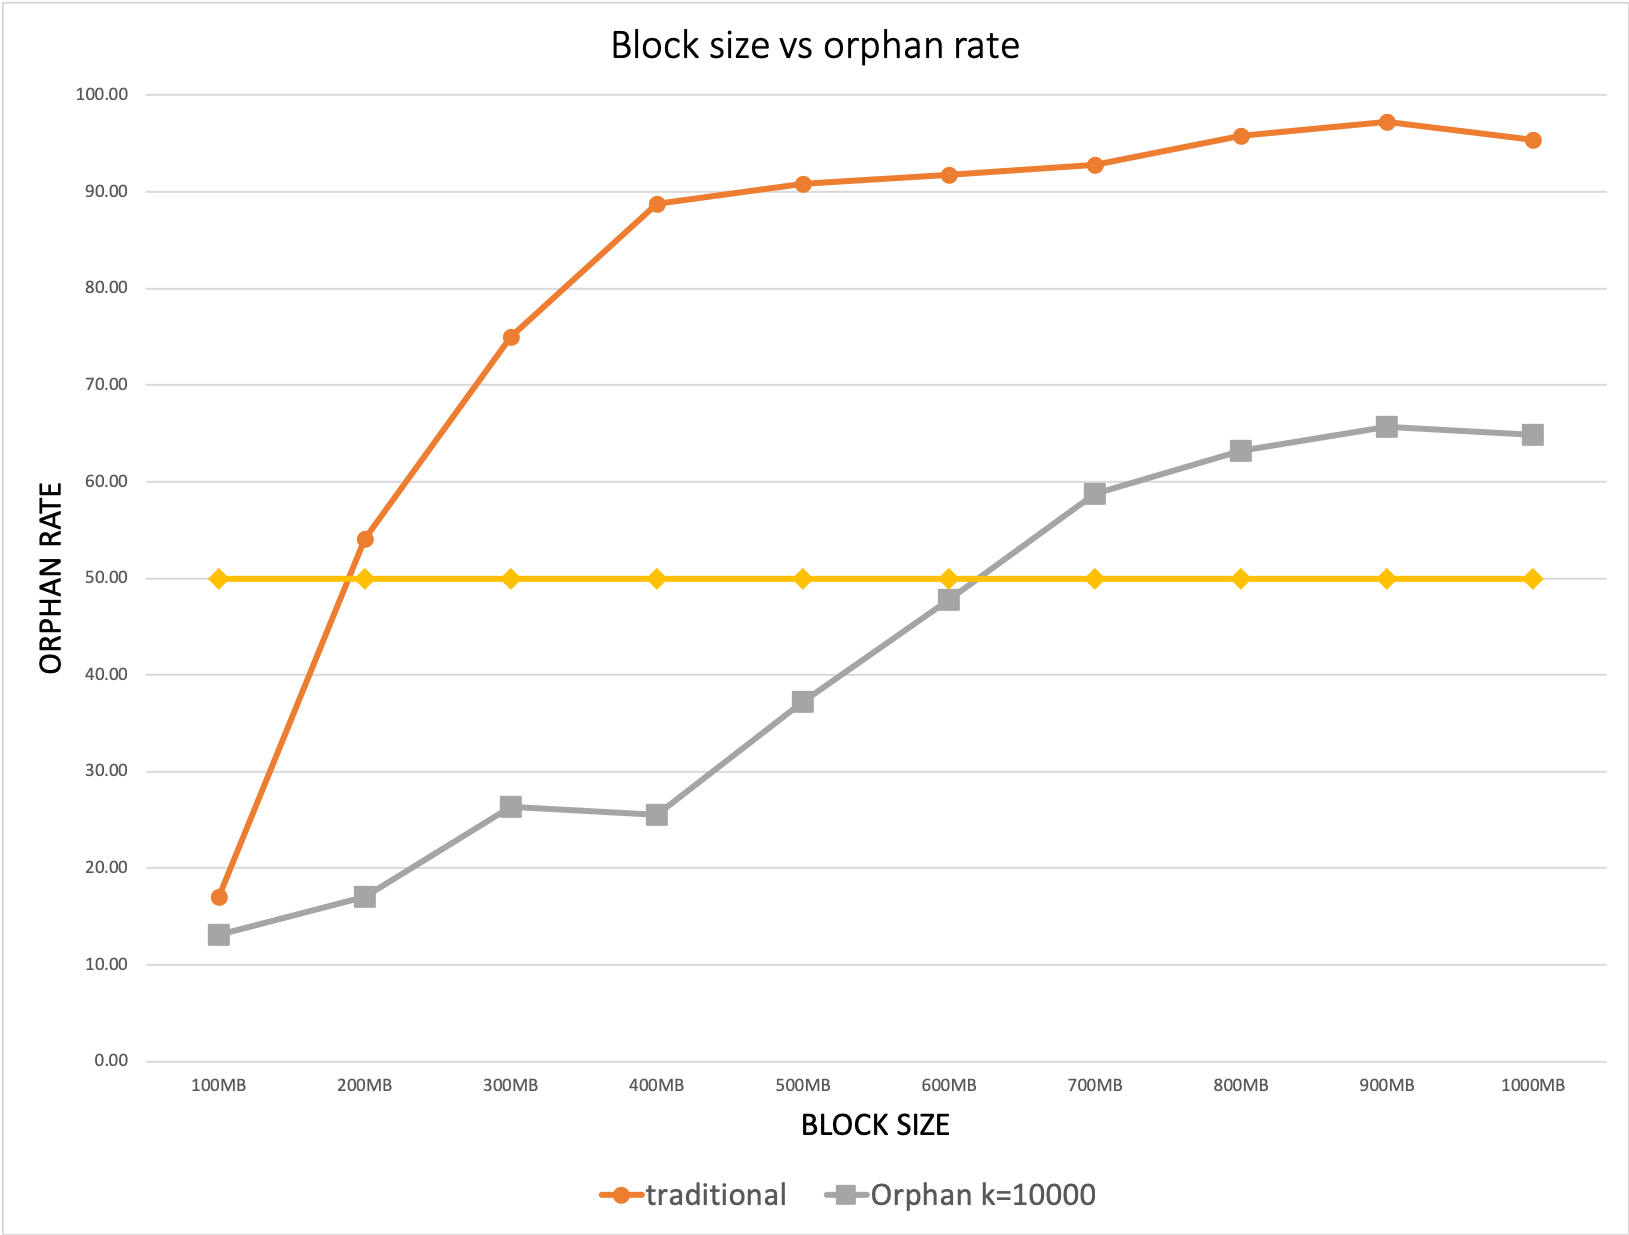
\includegraphics[width=1\columnwidth, height=.7\columnwidth]{files/orphan_10000.png}
     \centering
     \caption{Block Size vs Orphan Rate k=10000}
     \label{image: orphan_10000}
\end{figure}


From graphs \ref{image: orphan_10}, \ref{image: orphan_100}, \ref{image: orphan_1000}, \ref{image: orphan_10000} we can observe,

\begin{enumerate}
    \item The orphan rate in traditional relay reaches close to 97\%, that is that almost all blocks produced get orphaned when we run a 1 
        GigaByte simulation. That said, for all block sizes between 100MB and 1GB, the network is unable to maintain consensus.
    \item On the contrary, we see that when the data is aggregated from multiple 
        peers, the orphan rate is contained below 50\% for a 400MB block with \texttt{k} = 10 and for \texttt{k} between 100 and 10000, 
        the network maintains consensus below 600MB. 
\end{enumerate}

\subsubsection{Bandwidth}

\begin{enumerate}
    \item \textbf{average bandwidth} Average bandwidth used by both cases is
        similar in our simulations, however we are sending no overhead symbols.
        In case of lesser than k symbols received, we ask the peers again to
        send more symbols. 
    \item The total number of \texttt{getraptor} are
        significantly higher, by a factor of 2, in some cases 3. That is because
        of us sending multiple requests to aggregate one block. This doesn't
        affect the overall bandwidth utilization because the size of the request
        is 36 bytes each.
\end{enumerate}

\subsubsection{Median Block Propagation}

\begin{figure}
    \captionsetup{justification=centering}
    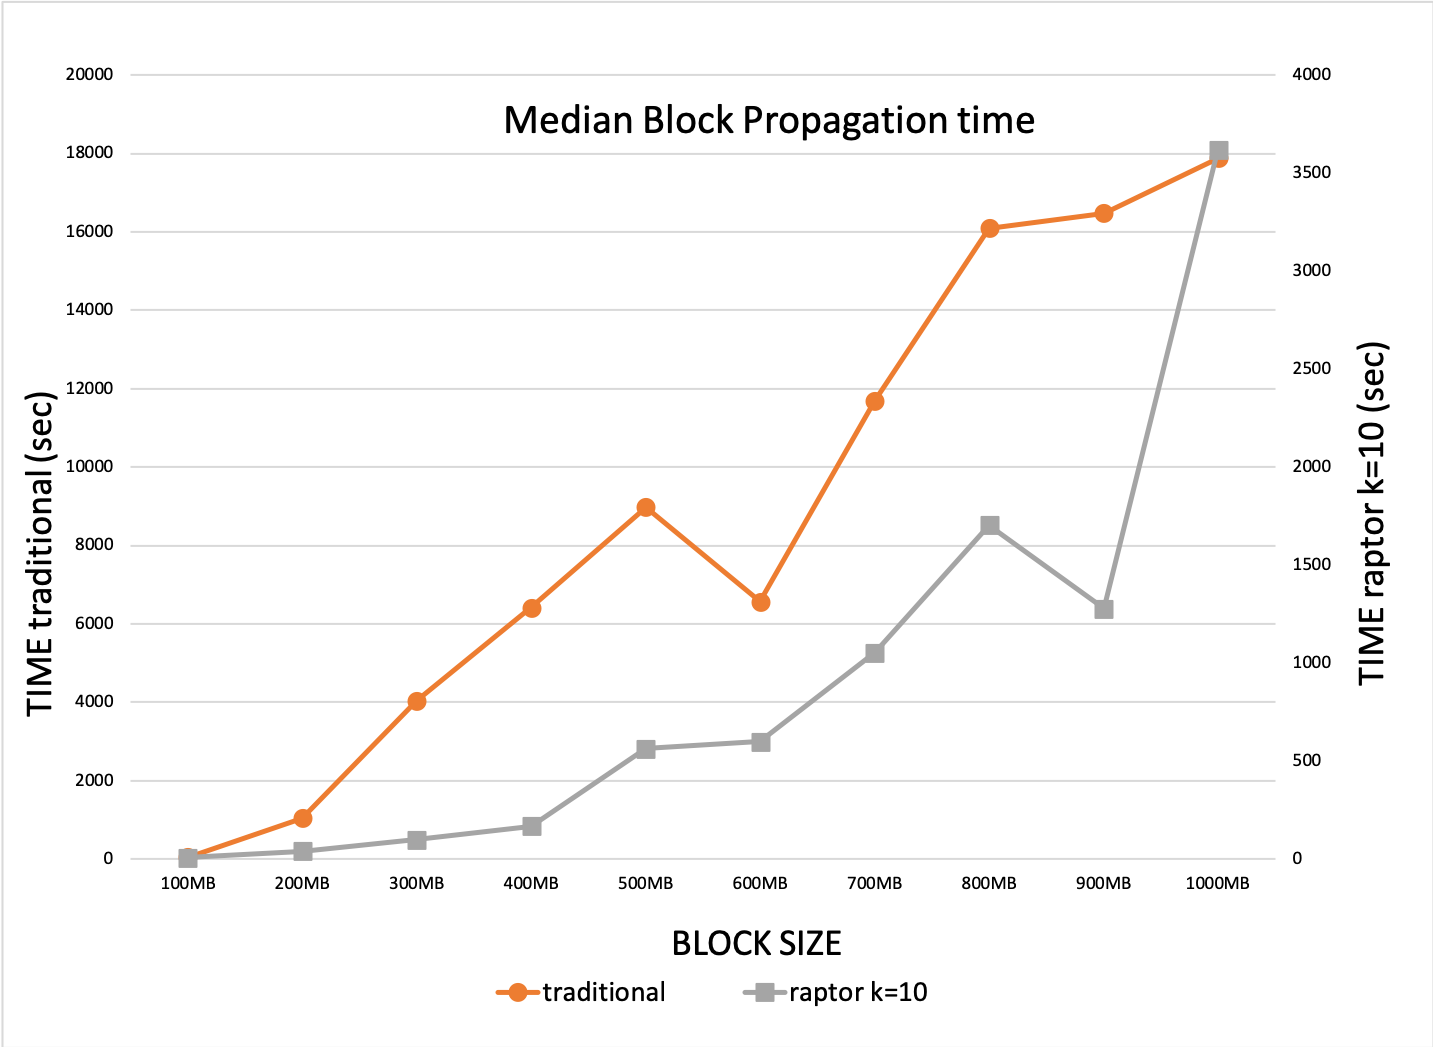
\includegraphics[width=1\columnwidth, height=.7\columnwidth]{files/propagation_10.png}
     \centering
     \caption{Median Block propagation k=10}
     \label{image: prop_10}
\end{figure}

\begin{figure}
    \captionsetup{justification=centering}
    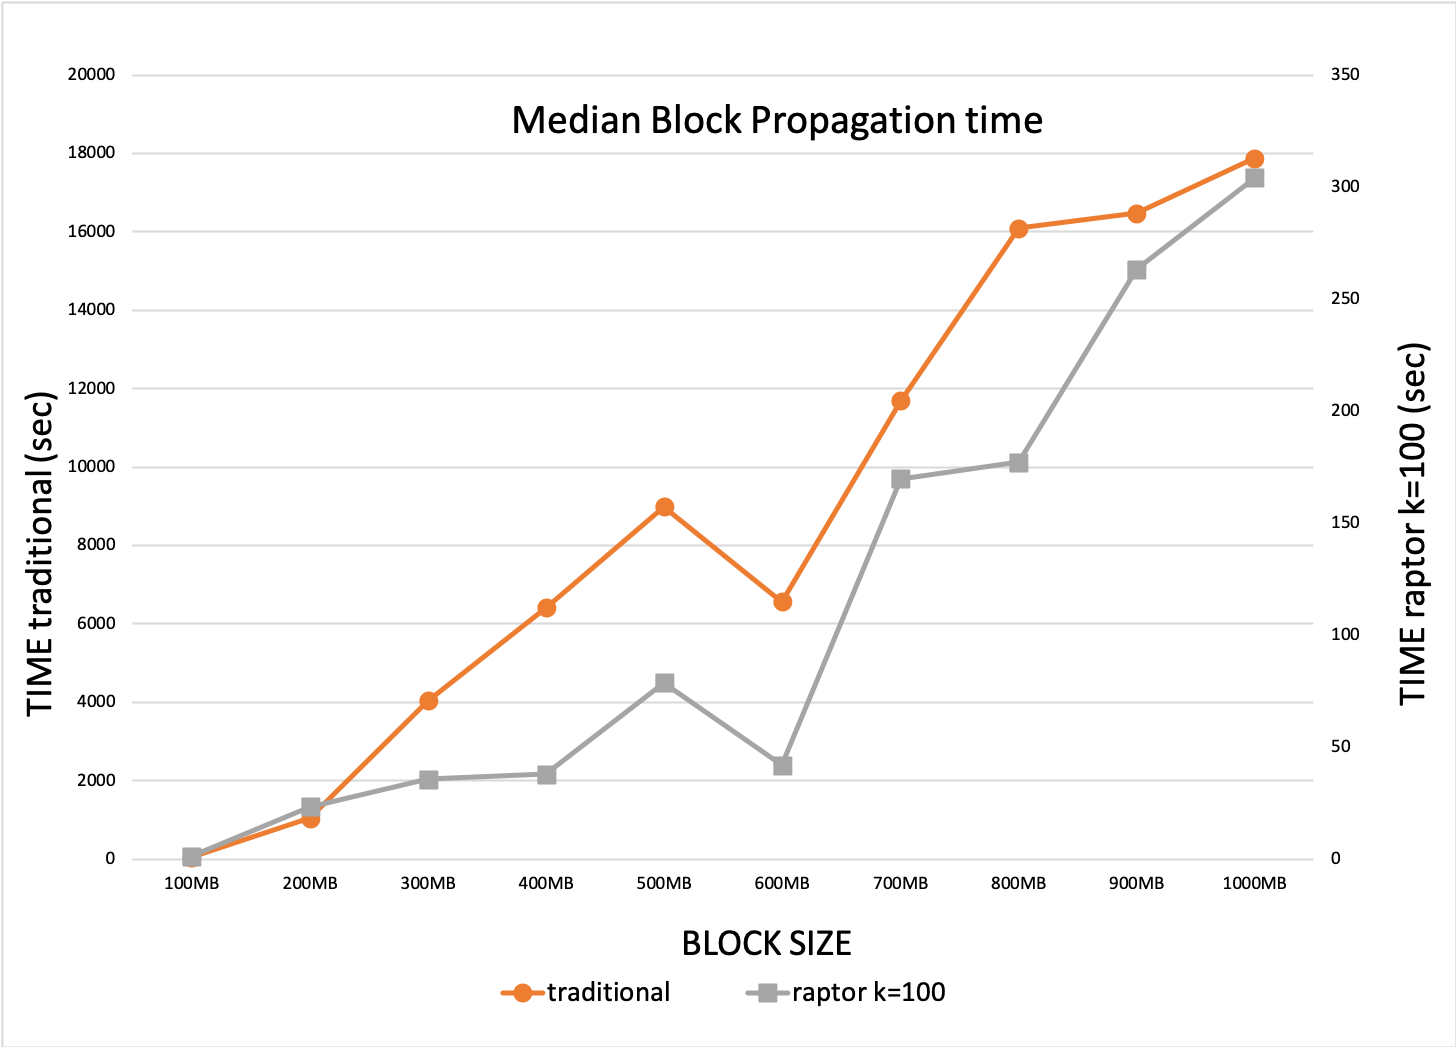
\includegraphics[width=1\columnwidth, height=.7\columnwidth]{files/propagation_100.png}
     \centering
     \caption{Median Block propagation k=100}
     \label{image: prop_100}
\end{figure}

\begin{figure}
    \captionsetup{justification=centering}
    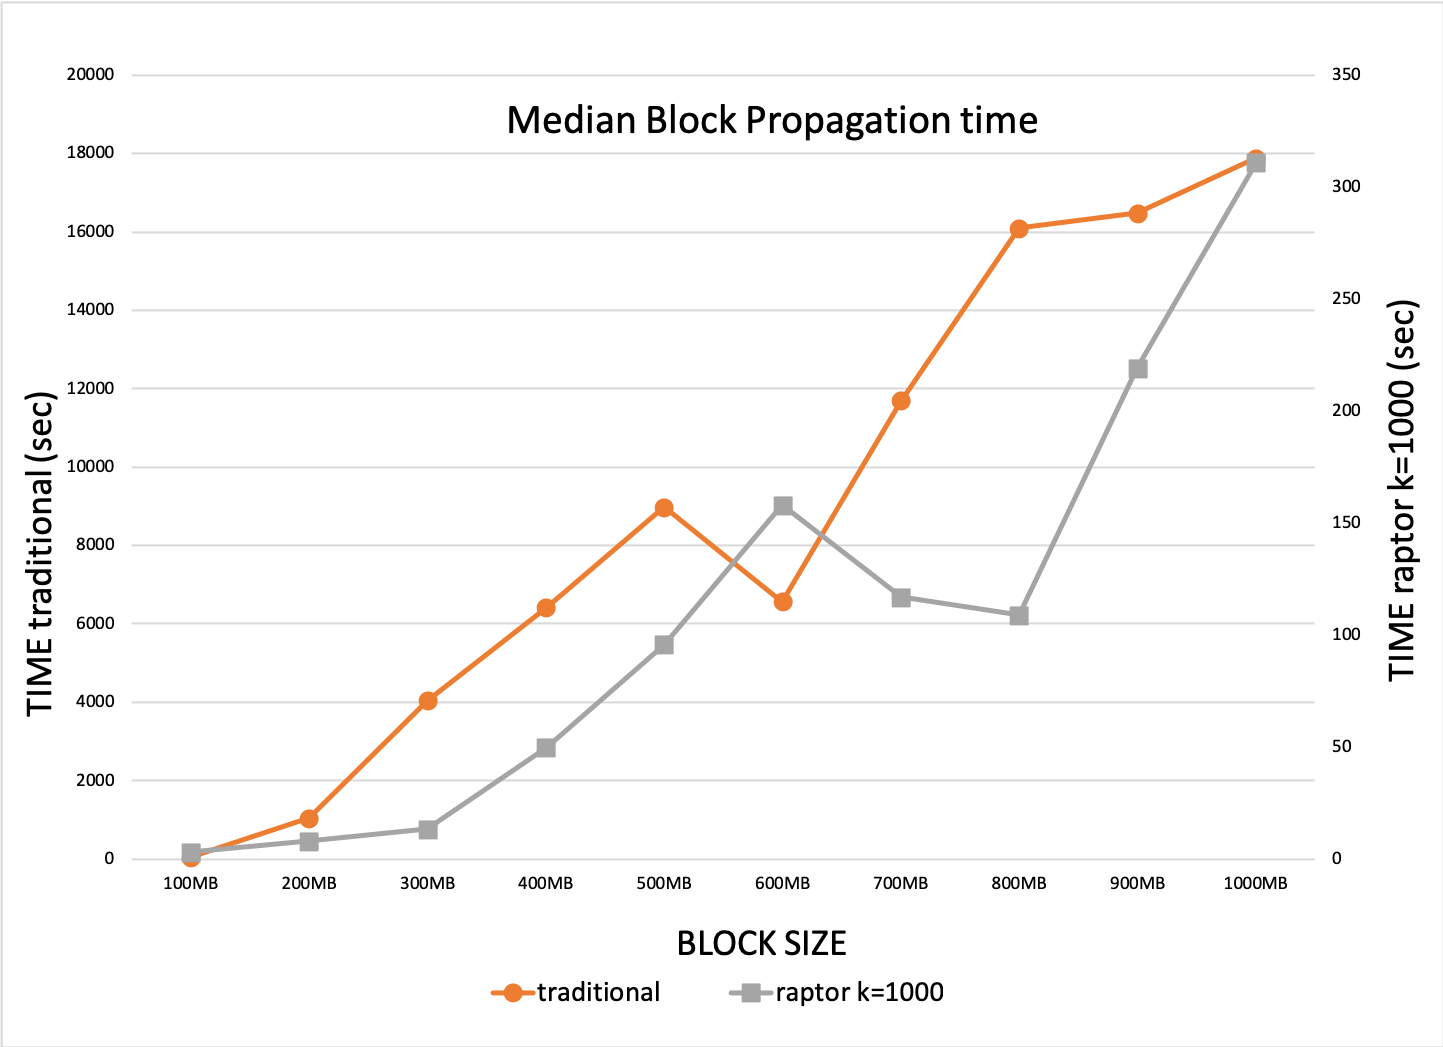
\includegraphics[width=1\columnwidth, height=.7\columnwidth]{files/propagation_1000.png}
     \centering
     \caption{Median Block propagation k=1000}
     \label{image: prop_1000}
\end{figure}

\begin{figure}
    \captionsetup{justification=centering}
    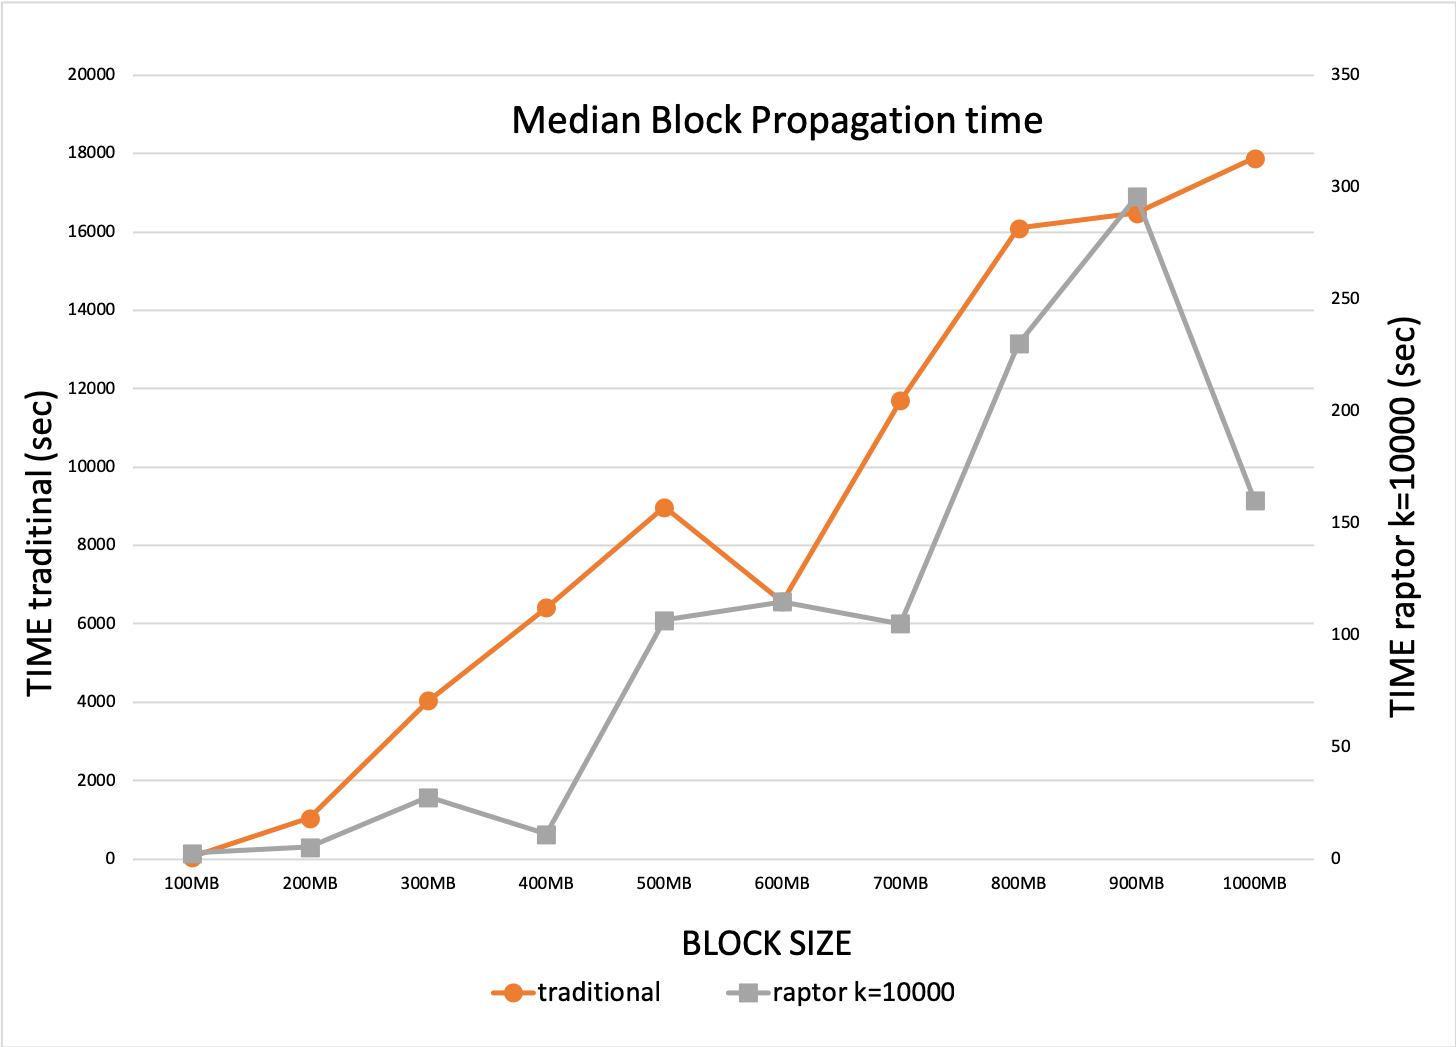
\includegraphics[width=1\columnwidth, height=.7\columnwidth]{files/propagation_10000.png}
     \centering
     \caption{Median Block propagation k=10000}
     \label{image: prop_10000}
\end{figure}

From graphs \ref{image: prop_10}, \ref{image: prop_100}, \ref{image: prop_1000}, \ref{image: prop_10000}, we can observe,

\begin{enumerate}
    \item The median block propagation for block sizes in traditional block propagation elevate above 2.5 minutes in 200MB block sizes, and that is noticeable in \ref{image: orphan_10} that 200MB blocks are not in consensus.
    \item The median block propagation remains below 2.5 minutes for Raptor Code Propagation till 400MB for \texttt{k=10} and remain below below 2.5 minutes for 600MB blocks for \texttt{k} between 100 and 10000. Therefore \ref{image: orphan_10} shows that consensus is maintained till 400MB blocks for \texttt{k=10} and \ref{image: orphan_100}, \ref{image: orphan_1000} and \ref{image: orphan_10000} show consensus is maintained for 600MB blocks for \texttt{k} values between 100 and 10000.
\end{enumerate}

